\documentclass[]{article}
\usepackage[labelfont=bf]{caption}
\usepackage[colorlinks=true,urlcolor=blue]{hyperref}
\usepackage{graphicx}
\usepackage{sidecap}
\setlength{\parindent}{0em}
\setlength{\parskip}{1em}
\graphicspath{{../figures/}}
\begin{document}

\title{a eZ idea of inversions}
\author{Jeff Ross-Ibarra, Wenbin Mei}
\maketitle

Chromosomes break. 
When they do, sometimes the cell's repair protocol doesn't work quite as expected, and occasionally the broken chunk of chromosome flips around before it is stuck back in place.  These changes, called inversions, can  have long played an important role in evolutionary genetics, serving as one of the \href{https://books.google.com/books?hl=en&lr=&id=PLSPhg3KPGgC&oi=fnd&pg=PA2&dq=Drosophila+Inversion+Polymorphism&ots=q3cP1SFpd-&sig=QFJcWW1RO6iSYEfqP-fx37R8hZw#v=onepage&q=Drosophila\%20Inversion\%20Polymorphism&f=false}{earliest genetic markers in \textit{Drosophila}}.  
Inversions can have functional consequences as well, including \href{}{disrupting gene function via breakage} or \href{}{modifying gene action by rearranging regulatory sequence}. 
Arguably the most important role of inversions, however, is their role in suppressing recombination and thus \href{}{fomenting adaptive divergence} and \href{}{introgression}
%<!-- kirkpatrick guerrero papers-->.
Because of this, inversions offer some of the coolest examples of single-locus traits, from \href{http://journals.plos.org/plosbiology/article?id=10.1371/journal.pbio.1000500}{perenniality in \textit{Mimulus}} to \href{http://www.nature.com/ng/journal/v48/n1/full/ng.3443.html}{mating behavior in birds}. 

\begin{SCfigure*}[][h!]   
   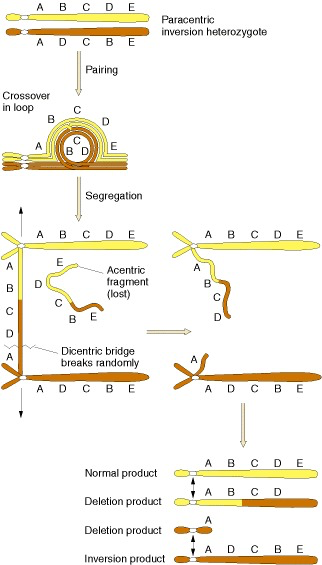
\includegraphics[width=0.3\linewidth]{ch17f16.png}
   \caption{ Inversion loops and the consequences of crossing over in an individual heterozygous for an inversion polymorphism. Image from \href{http://www.ncbi.nlm.nih.gov/books/NBK22042//}{Griffiths et al. 2000 via NCBI}. Video and additional information available at source.} 
    \label{fig:loop}
\end{SCfigure*}

It's not all melodies and monkeyflowers, however --- inversions come with a cost.  
In order for chromosomes to pair correctly in individuals heterozygous for an inversion, the chromosomes have to perform a bit of cytological gymnastics.  
A meiotic crossover in the middle of this tangle can then lead to Bad Things (Fig. \ref{fig:loop}).  
This heterozygous cost should limit the ability of new inversions to spread and explain why inversions are relatively rare. 

But what if there wasn't a cost? 
Much of the evidence for inversion loops and the consequences of crossing over comes from a few model systems, but is it universal? 
Turns out the answer is no.  
In maize, for example, cytological work by \href{http://www.ncbi.nlm.nih.gov/pmc/articles/PMC1211081/}{Marjorie Maguire} has shown that even for large inversions --- say, making up nearly 20\% of the length of a chromosome --- most the time inversion heterozygotes never make a loop].  
Instead, almost half the time the chromosomes just zip right up, essentially ignoring the lack of homology (Fig. \ref{fig:maguire}).  
Another 20\% of the time the genome seems to recognize the lack of homology and decide not to pair at all, resulting in a bubble of sorts.  
Only a third of the time does a loop even form. 
And because inversion breakpoints tend to occur in repetitive regions of the genome with low recombination rates, the chance of a crossover in heterozygotes for even a large inversion are relatively small. 
Crossing over in a \href{http://www.genetics.org/content/191/3/883.short}{50 megabase inversion} (that's more than a third of the length of the entire \textit{Arabidopsis} genome for those keeping score), for example, may only occur in as few as 3\% of meioses.

\begin{figure*}[h]   
   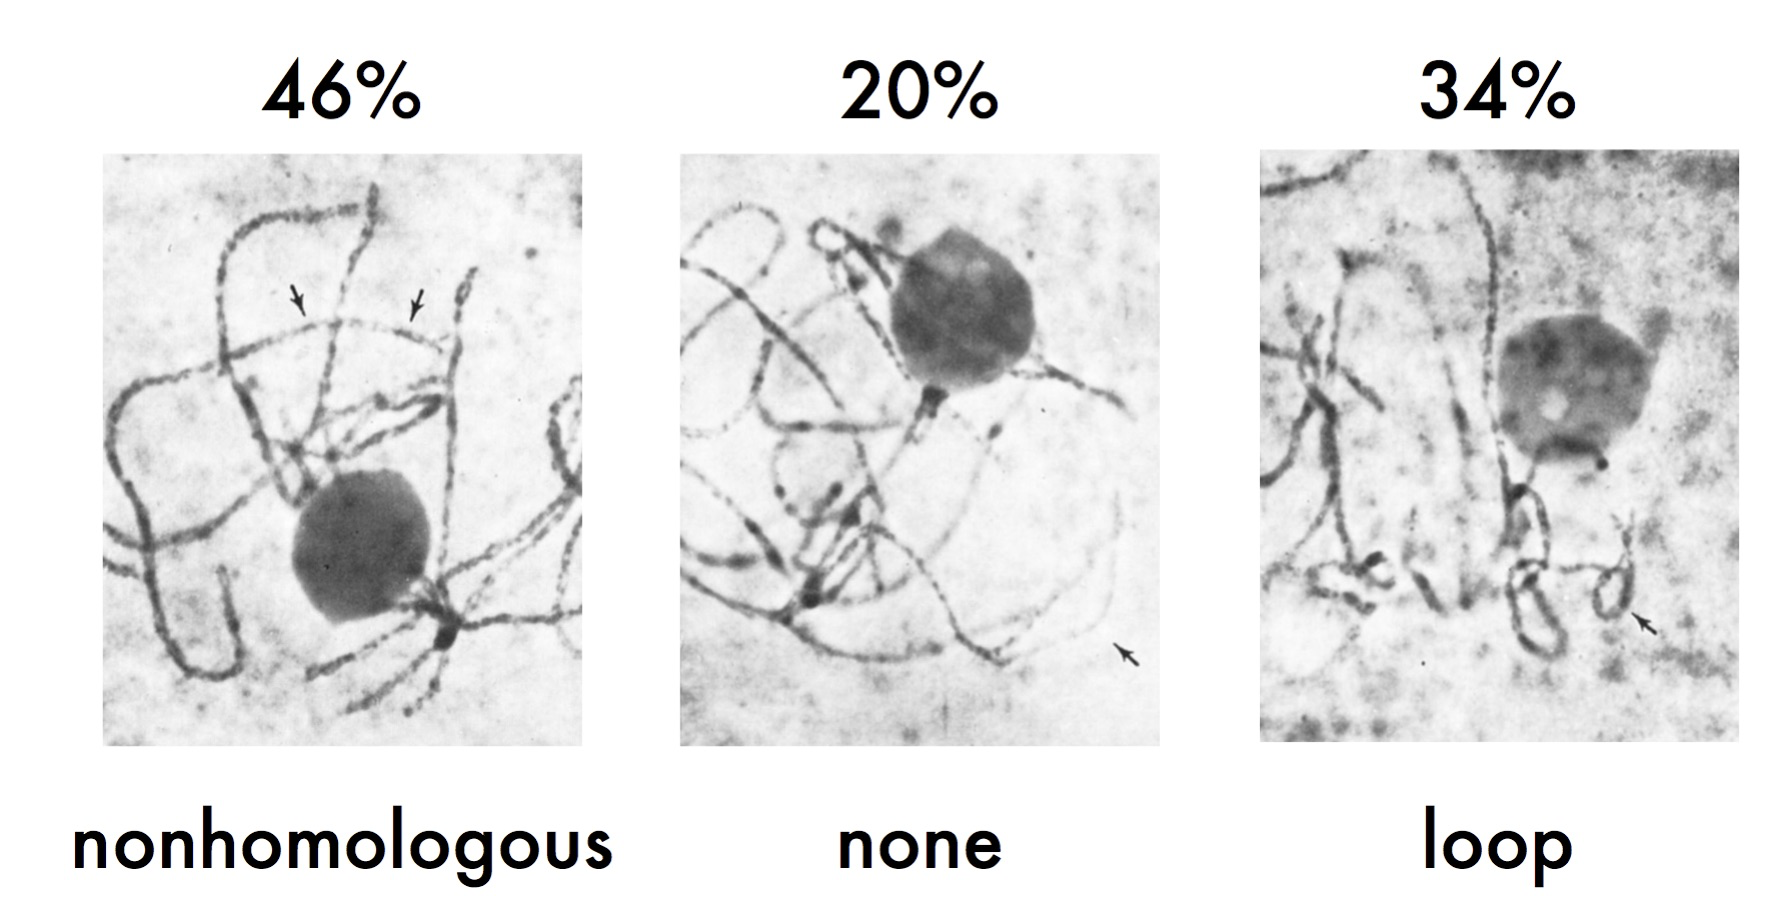
\includegraphics[width=0.9\linewidth]{maguire_inversions.png}
   \caption{ Inversion heterozygotes in \textit{Zea mays} and the consequences of crossing over in an individual heterozygous for an inversion polymorphism. Images from \href{http://www.ncbi.nlm.nih.gov/pmc/articles/PMC1211081/}{Maguire 1966}.} 
    \label{fig:maguire}
\end{figure*}

So what's the difference? Why are inversions less problematic in maize than *Drosophila*? Genome size! (Readers may be excused for imagining a trend in my blog posts.) 
The maize genome is 2500Mb in size, and includes tens of thousands of full-length transposable elements.  
Much of this nongenic DNA is not shared between maize lines: an early genomic analysis of BAC sequences found that two popular inbred lines \href{http://www.ncbi.nlm.nih.gov/pubmed/15659640}{only share ~50\% of the DNA sequence} in many regions of the genome.  
A cell sensitive to such extreme lack of homology would be unable to undergo normal chromosome pairing.  
Presumably the maize genome has learned to cope with this difficulty, and it seems likely that whatever mechanisms allow the genome to pair chromosomes with such substantial differences also allows it to deal with a lack of homology due to inversions as well. 
If so, we might expect inversions to be more common in complex genomes such as maize. 
Indeed, simple surveys of a handful of population using relatively low-density genotyping easily pick up \href{http://gbe.oxfordjournals.org/content/5/9/1594.short}{multiple} megabase-scale inversions.  
Smaller inversions will be harder to detect, of course, but also less likely to be disrupted by crossing over and probably much more abundant in the genome.  
And because maize is a relatively average plant genome, it's quite likely that inversion polymorphisms are extremely common in plants. {\bf Let's go find them.}

\end{document}